%% LyX 2.1.0 created this file.  For more info, see http://www.lyx.org/.
%% Do not edit unless you really know what you are doing.
\documentclass[english,11pt,oneside,final]{fithesis2}
\usepackage[T1]{fontenc}
\usepackage[utf8]{inputenc}
\setcounter{secnumdepth}{3}
\setcounter{tocdepth}{3}
\usepackage{graphicx}

\makeatletter

%%%%%%%%%%%%%%%%%%%%%%%%%%%%%% LyX specific LaTeX commands.

\thesistitle{Návrh a implementace rozhraní pro monitorování komponenty Engine
systému Perun }
\thesissubtitle{Bakalářská práce}
\thesisstudent{Jana Čecháčková}
\thesiswoman{false}
\thesisuniversity{Masarykova univerzita}
\thesisfaculty{Fakulta informatiky}
\thesislogo{fi-logo}
\thesisadvisor{Mgr. Slávek Licehammer}
\thesisyear{Brno, jaro 2014}
\thesislang{cs}

%%%%%%%%%%%%%%%%%%%%%%%%%%%%%% Textclass specific LaTeX commands.

\newcommand{\TitlePages}{\ThesisTitlePage\FrontMatter}

\makeatother

\usepackage{babel}
\begin{document}
\TitlePages
\begin{ThesisDeclaration}
\DeclarationText
\AdvisorName\end{ThesisDeclaration}
\begin{ThesisKeyWords}
Smrk, žížala, krabice.\end{ThesisKeyWords}
\begin{ThesisThanks}
Rád bych na tomto místě poděkoval svému vedoucímu...
\end{ThesisThanks}
\noindent \tableofcontents{}

\noindent \MainMatter


\chapter{Žížala zelená}

\begin{figure}
\begin{centering}
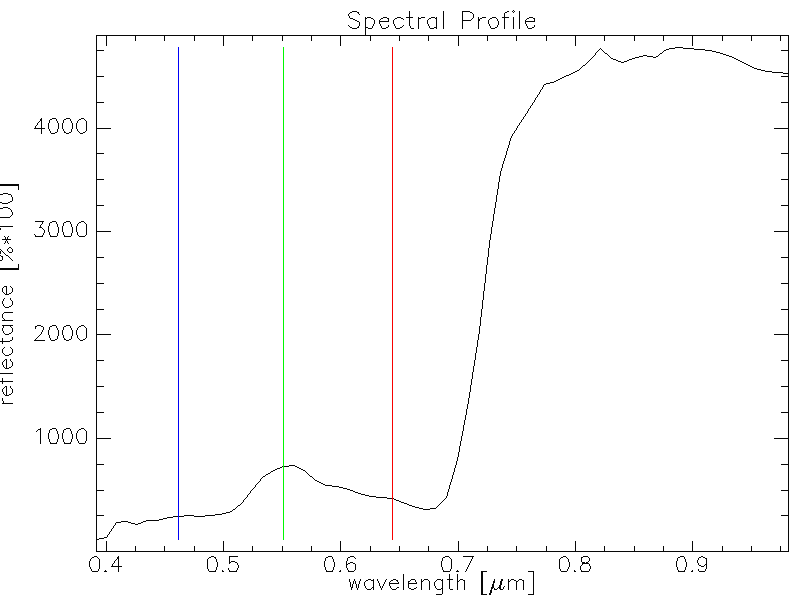
\includegraphics[width=6cm]{spectral-signal-tree}
\par\end{centering}

\protect\caption{Vobrázek}
\end{figure}

\end{document}
